\documentclass{standalone}
\usepackage{tikz}
\usetikzlibrary{patterns}
\usetikzlibrary{positioning}
\usetikzlibrary{patterns, positioning}
\usetikzlibrary{shapes.misc}
\usepackage[outline]{contour}
\contourlength{1.5pt} 
\usepackage[sfdefault]{ClearSans}

\begin{document}
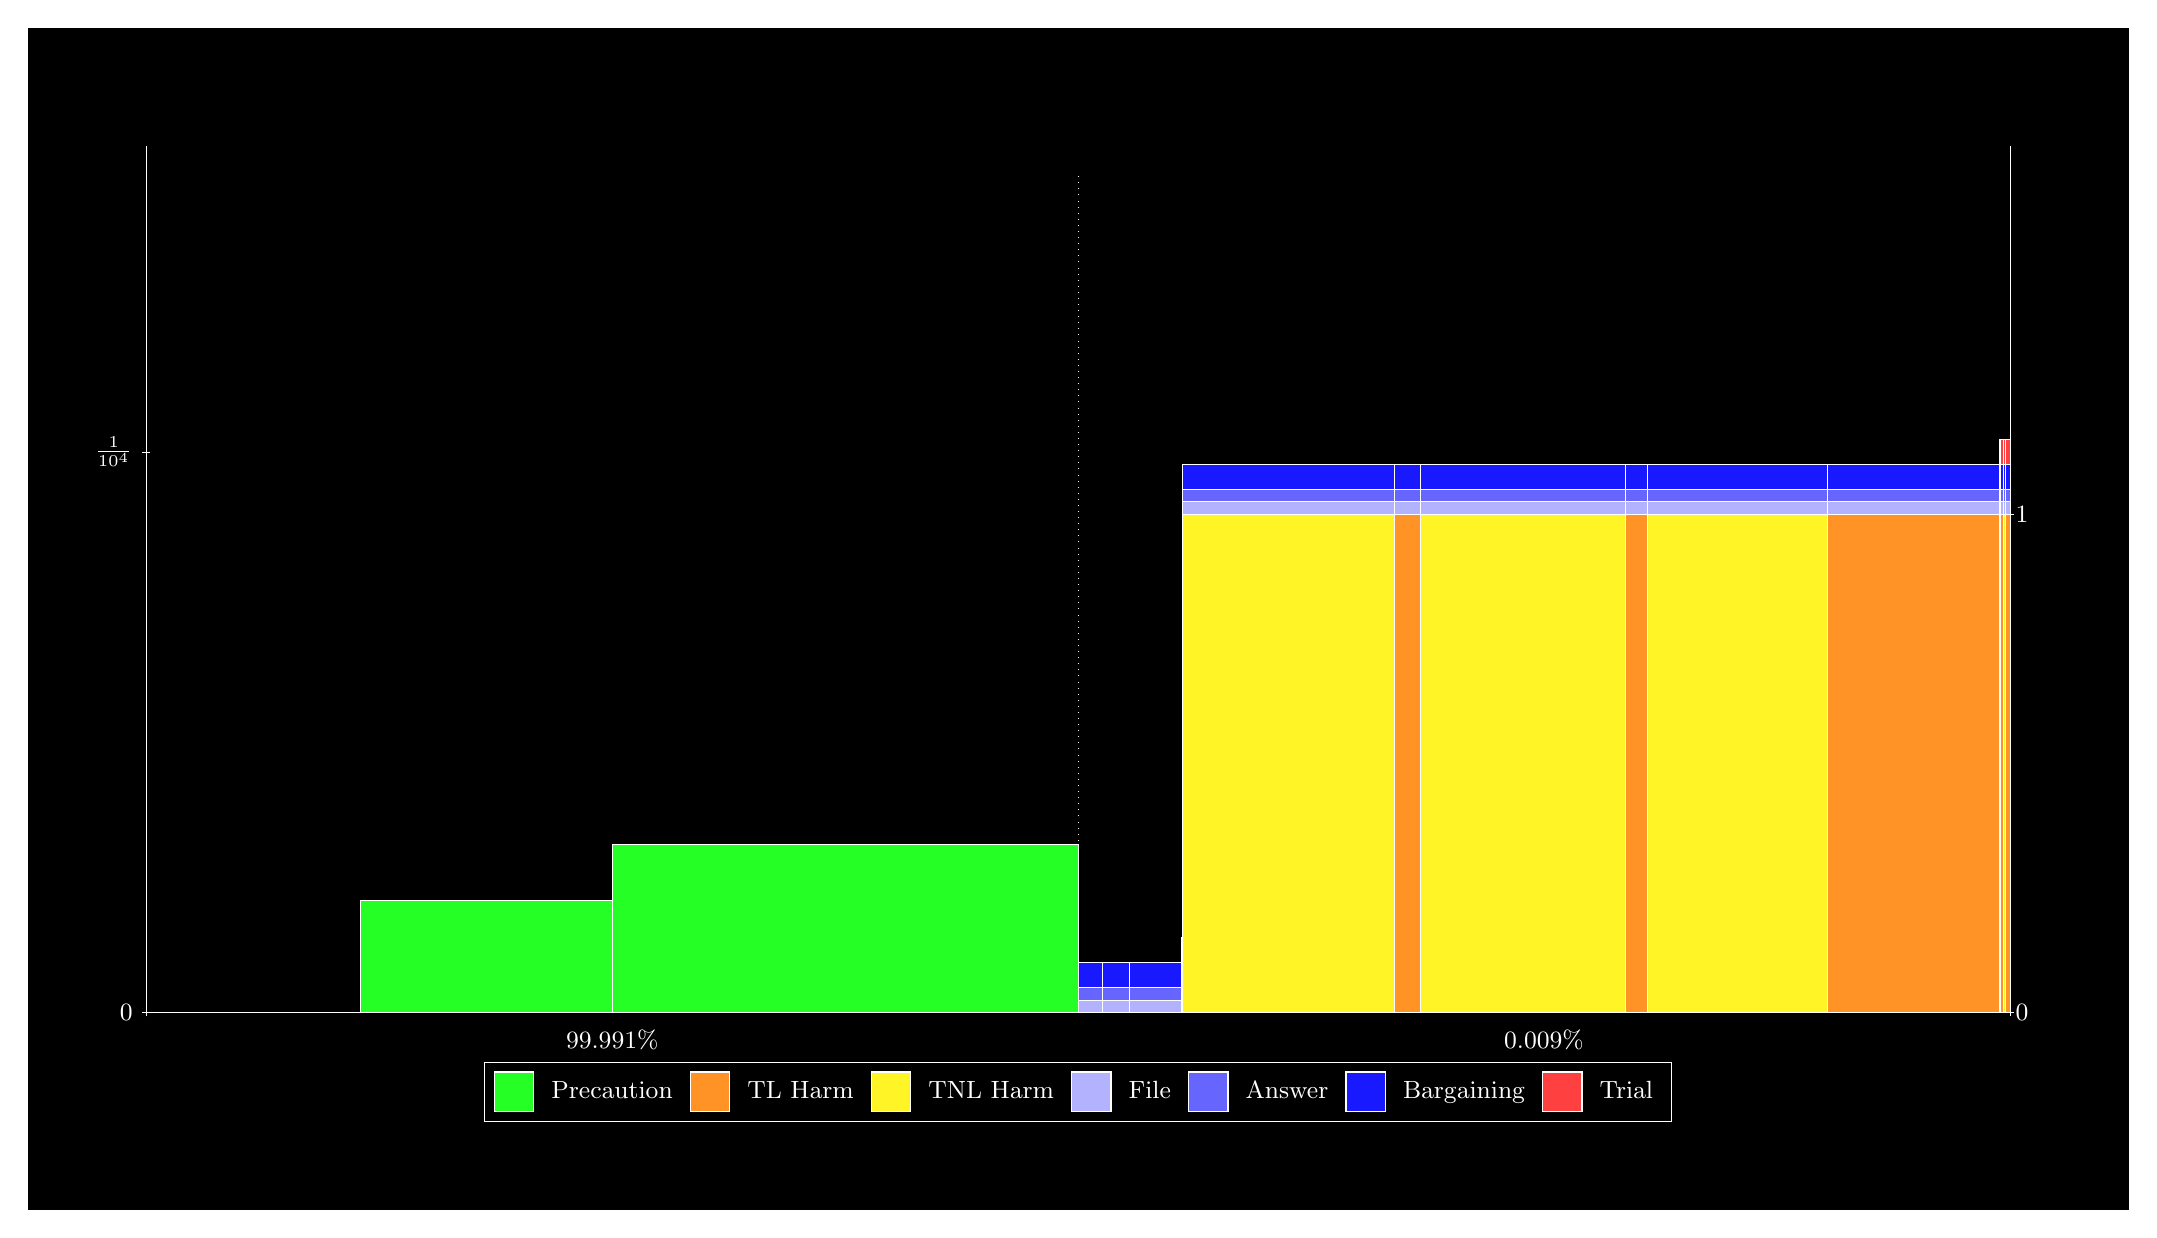
\begin{tikzpicture}
\draw[fill=black] (0,0) rectangle (26.667,15);
\draw[fill=green!85,draw=white,very thin] (4.2218,2.5) rectangle (7.4166,3.9241);
\draw[fill=green!85,draw=white,very thin] (7.4166,2.5) rectangle (13.333,4.6362);
\draw[fill=blue!30,draw=white,very thin] (13.333,2.5) rectangle (13.635,2.6583);
\draw[fill=blue!60,draw=white,very thin] (13.333,2.6583) rectangle (13.635,2.8165);
\draw[fill=blue!90,draw=white,very thin] (13.333,2.8165) rectangle (13.635,3.133);
\draw[fill=green!85,draw=white,very thin] (13.635,2.5) rectangle (13.983,2.5001);
\draw[fill=blue!30,draw=white,very thin] (13.635,2.5001) rectangle (13.983,2.6584);
\draw[fill=blue!60,draw=white,very thin] (13.635,2.6584) rectangle (13.983,2.8166);
\draw[fill=blue!90,draw=white,very thin] (13.635,2.8166) rectangle (13.983,3.1332);
\draw[fill=green!85,draw=white,very thin] (13.983,2.5) rectangle (14.649,2.5002);
\draw[fill=blue!30,draw=white,very thin] (13.983,2.5002) rectangle (14.649,2.6585);
\draw[fill=blue!60,draw=white,very thin] (13.983,2.6585) rectangle (14.649,2.8167);
\draw[fill=blue!90,draw=white,very thin] (13.983,2.8167) rectangle (14.649,3.1332);
\draw[fill=green!85,draw=white,very thin] (14.649,2.5) rectangle (14.66,2.5001);
\draw[fill=blue!30,draw=white,very thin] (14.649,2.5001) rectangle (14.66,2.6584);
\draw[fill=blue!60,draw=white,very thin] (14.649,2.6584) rectangle (14.66,2.8166);
\draw[fill=blue!90,draw=white,very thin] (14.649,2.8166) rectangle (14.66,3.1332);
\draw[fill=red!75,draw=white,very thin] (14.649,3.1332) rectangle (14.66,3.4497);
\draw[fill=yellow!85,draw=white,very thin] (14.66,2.5) rectangle (17.347,8.8304);
\draw[fill=blue!30,draw=white,very thin] (14.66,8.8304) rectangle (17.347,8.9887);
\draw[fill=blue!60,draw=white,very thin] (14.66,8.9887) rectangle (17.347,9.147);
\draw[fill=blue!90,draw=white,very thin] (14.66,9.147) rectangle (17.347,9.4635);
\draw[fill=orange!85,draw=white,very thin] (17.347,2.5) rectangle (17.681,8.8304);
\draw[fill=blue!30,draw=white,very thin] (17.347,8.8304) rectangle (17.681,8.9887);
\draw[fill=blue!60,draw=white,very thin] (17.347,8.9887) rectangle (17.681,9.147);
\draw[fill=blue!90,draw=white,very thin] (17.347,9.147) rectangle (17.681,9.4635);
\draw[fill=green!85,draw=white,very thin] (17.681,2.5) rectangle (20.28,2.5001);
\draw[fill=yellow!85,draw=white,very thin] (17.681,2.5001) rectangle (20.28,8.8306);
\draw[fill=blue!30,draw=white,very thin] (17.681,8.8306) rectangle (20.28,8.9888);
\draw[fill=blue!60,draw=white,very thin] (17.681,8.9888) rectangle (20.28,9.1471);
\draw[fill=blue!90,draw=white,very thin] (17.681,9.1471) rectangle (20.28,9.4636);
\draw[fill=green!85,draw=white,very thin] (20.28,2.5) rectangle (20.562,2.5001);
\draw[fill=orange!85,draw=white,very thin] (20.28,2.5001) rectangle (20.562,8.8306);
\draw[fill=blue!30,draw=white,very thin] (20.28,8.8306) rectangle (20.562,8.9888);
\draw[fill=blue!60,draw=white,very thin] (20.28,8.9888) rectangle (20.562,9.1471);
\draw[fill=blue!90,draw=white,very thin] (20.28,9.1471) rectangle (20.562,9.4636);
\draw[fill=green!85,draw=white,very thin] (20.562,2.5) rectangle (22.851,2.5002);
\draw[fill=yellow!85,draw=white,very thin] (20.562,2.5002) rectangle (22.851,8.8306);
\draw[fill=blue!30,draw=white,very thin] (20.562,8.8306) rectangle (22.851,8.9889);
\draw[fill=blue!60,draw=white,very thin] (20.562,8.9889) rectangle (22.851,9.1472);
\draw[fill=blue!90,draw=white,very thin] (20.562,9.1472) rectangle (22.851,9.4637);
\draw[fill=green!85,draw=white,very thin] (22.851,2.5) rectangle (25.038,2.5002);
\draw[fill=orange!85,draw=white,very thin] (22.851,2.5002) rectangle (25.038,8.8306);
\draw[fill=blue!30,draw=white,very thin] (22.851,8.8306) rectangle (25.038,8.9889);
\draw[fill=blue!60,draw=white,very thin] (22.851,8.9889) rectangle (25.038,9.1472);
\draw[fill=blue!90,draw=white,very thin] (22.851,9.1472) rectangle (25.038,9.4637);
\draw[fill=yellow!85,draw=white,very thin] (25.038,2.5) rectangle (25.047,8.8304);
\draw[fill=blue!30,draw=white,very thin] (25.038,8.8304) rectangle (25.047,8.9887);
\draw[fill=blue!60,draw=white,very thin] (25.038,8.9887) rectangle (25.047,9.147);
\draw[fill=blue!90,draw=white,very thin] (25.038,9.147) rectangle (25.047,9.4635);
\draw[fill=red!75,draw=white,very thin] (25.038,9.4635) rectangle (25.047,9.78);
\draw[fill=orange!85,draw=white,very thin] (25.047,2.5) rectangle (25.079,8.8304);
\draw[fill=blue!30,draw=white,very thin] (25.047,8.8304) rectangle (25.079,8.9887);
\draw[fill=blue!60,draw=white,very thin] (25.047,8.9887) rectangle (25.079,9.147);
\draw[fill=blue!90,draw=white,very thin] (25.047,9.147) rectangle (25.079,9.4635);
\draw[fill=red!75,draw=white,very thin] (25.047,9.4635) rectangle (25.079,9.78);
\draw[fill=green!85,draw=white,very thin] (25.079,2.5) rectangle (25.105,2.5001);
\draw[fill=yellow!85,draw=white,very thin] (25.079,2.5001) rectangle (25.105,8.8306);
\draw[fill=blue!30,draw=white,very thin] (25.079,8.8306) rectangle (25.105,8.9888);
\draw[fill=blue!60,draw=white,very thin] (25.079,8.9888) rectangle (25.105,9.1471);
\draw[fill=blue!90,draw=white,very thin] (25.079,9.1471) rectangle (25.105,9.4636);
\draw[fill=red!75,draw=white,very thin] (25.079,9.4636) rectangle (25.105,9.7801);
\draw[fill=green!85,draw=white,very thin] (25.105,2.5) rectangle (25.167,2.5001);
\draw[fill=orange!85,draw=white,very thin] (25.105,2.5001) rectangle (25.167,8.8306);
\draw[fill=blue!30,draw=white,very thin] (25.105,8.8306) rectangle (25.167,8.9888);
\draw[fill=blue!60,draw=white,very thin] (25.105,8.9888) rectangle (25.167,9.1471);
\draw[fill=blue!90,draw=white,very thin] (25.105,9.1471) rectangle (25.167,9.4636);
\draw[fill=red!75,draw=white,very thin] (25.105,9.4636) rectangle (25.167,9.7801);
\draw[white,very thin] (1.5,2.5) -- (1.5,13.5);
\draw[white,very thin] (1.45,2.5) -- (1.55,2.5);
\node[font=\small,text=white, anchor=east] at (1.45, 2.5) {0};
\draw[white,very thin] (1.45,9.6206) -- (1.55,9.6206);
\node[font=\small,text=white, anchor=east] at (1.45, 9.6206) {$\frac{1}{10^{4}}$};

\draw[white,dotted,very thin] (13.333,2.83) -- (13.333,13.17);
\draw[white,very thin] (25.167,2.5) -- (25.167,13.5);
\draw[white,very thin] (25.117,2.5) -- (25.217,2.5);
\node[font=\small,text=white, anchor=west] at (25.117, 2.5) {0};
\draw[white,very thin] (25.117,8.8304) -- (25.217,8.8304);
\node[font=\small,text=white, anchor=west] at (25.117, 8.8304) {1};

\draw[white,very thin] (1.5,2.5) -- (25.167,2.5);
\draw[white,very thin] (1.5,2.45) -- (1.5,2.55);
\node[font=\small,text=white, anchor=north] at (1.5, 2.45) {};
\draw[white,very thin] (25.167,2.45) -- (25.167,2.55);
\node[font=\small,text=white, anchor=north] at (25.167, 2.45) {};

\node[font=\small,text=white,anchor=south] at (7.4167, 1.9) {99.991\%};
\node[font=\small,text=white,anchor=south] at (19.25, 1.9) {0.009\%};
\draw (13.3333,2.5) node (B) {};
\begin{scope}[align=center]
\matrix[scale=0.5,draw=white,below=0.5cm of B,nodes={draw},column sep=0.1cm]{
\node[rectangle,draw,minimum width=0.5cm,minimum height=0.5cm,fill=green!85]{}; & \node[draw=none,font=\small,text=white]{Precaution}; &
\node[rectangle,draw,minimum width=0.5cm,minimum height=0.5cm,fill=orange!85]{}; & \node[draw=none,font=\small,text=white]{TL Harm}; &
\node[rectangle,draw,minimum width=0.5cm,minimum height=0.5cm,fill=yellow!85]{}; & \node[draw=none,font=\small,text=white]{TNL Harm}; &
\node[rectangle,draw,minimum width=0.5cm,minimum height=0.5cm,fill=blue!30]{}; & \node[draw=none,font=\small,text=white]{File}; &
\node[rectangle,draw,minimum width=0.5cm,minimum height=0.5cm,fill=blue!60]{}; & \node[draw=none,font=\small,text=white]{Answer}; &
\node[rectangle,draw,minimum width=0.5cm,minimum height=0.5cm,fill=blue!90]{}; & \node[draw=none,font=\small,text=white]{Bargaining}; &
\node[rectangle,draw,minimum width=0.5cm,minimum height=0.5cm,fill=red!75]{}; & \node[draw=none,font=\small,text=white]{Trial}; \\\\
};\end{scope}

\end{tikzpicture}
\end{document}